\documentclass[logo,reportComp]{thesis}
\usepackage[python,pseudo]{mypackage}
\usepackage{relsize}

\setcounter{secnumdepth}{4}
\titleformat{\paragraph}{\bfseries}{\alph{paragraph})~~}{0em}{}
\titlespacing*{\paragraph}{0pt}{0pt}{0pt}[0pt]

\title{自然语言处理}
\subtitle{期末大项目:基于深度学习的中英机器翻译}
\school{数据科学与计算机学院}
\author{陈鸿峥}
\classname{17大数据与人工智能}
\stunum{17341015}
\headercontext{自然语言处理作业}

\let\emph\relax % there's no \RedeclareTextFontCommand
\DeclareTextFontCommand{\emph}{\kaiti\em}
\AtBeginEnvironment{quote}{\kaiti\small}

\newcommand{\cfbox}[2]{%
    \colorlet{currentcolor}{.}%
    {\color{#1}%
    \fbox{\color{currentcolor}#2}}%
}

\def\unidia{${\mathlarger{\mathlarger{\Diamond}}}\mathllap{?\,}$}

\begin{document}

\maketitle
\tableofcontents

\newpage

本次实验主要分为预处理、模型搭建、模型训练、模型预测几个部分,下面将详细进行说明。

\section{预处理}
由于原始数据集数据没有进行清洗,因此在预处理阶段做的工作非常的多。

\subsection{数据读入}
本次实验使用\verb'dataset_10000'的数据集,主要有以下几个文件。
\begin{table}[H]
\centering
\begin{tabular}{|c|c|c|}\hline
训练集 & X\_train & \verb'train_source_8000.txt'\\\hline
训练集 & Y\_train & \verb'train_target_8000.txt'\\\hline
测试集 & X\_test & \verb'test_source_1000.txt'\\\hline
测试集 & Y\_test & \verb'test_target_1000.txt'\\\hline
验证集 & X\_dev & \verb'dev_source_1000.txt'\\\hline
验证集 & Y\_dev & \verb'dev_target_1000.txt'\\\hline
\end{tabular}
\end{table}

在每一组数据集的每一行都是一对平行语料,比如下面的例子。
\begin{quote}
巴黎-随着经济危机不断加深和蔓延,整个世界一直在寻找历史上的类似事件希望有助于我们了解目前正在发生的情况。\\
PARIS -- As the economic crisis deepens and widens, the world has been searching for historical analogies to help us understand what has been happening.
\end{quote}

因此,为了更好组织这些平行语料,可以采用\verb'zip'语句将源语料的句子和目标语料的句子进行组合,逐行读入后对这些句子进行字符串处理,核心代码如下。
\begin{lstlisting}
for i,(src_line,dst_line) in enumerate(zip(src_file,dst_file),1):
    src = src_line.splitlines()[0]
    dst = dst_line.splitlines()[0]
    norm_src = Lang.normalizeString(src,"zh")
    norm_dst = Lang.normalizeString(dst,"en")
    src_lang.addSentence(norm_src)
    dst_lang.addSentence(norm_dst)
    pairs.append([norm_src,norm_dst])
\end{lstlisting}

可以清晰见到,这里主要分为三个步骤:
\begin{enumerate}
\item 读入一行,注意这里需要用\verb'splitlines'将行末空格去除
\item 调用normalizeString对源/目标句子进行处理(见\ref{sub:string}节)
\item 将处理后的句子添加入对应类中进行存储
\end{enumerate}

\subsection{字符串处理}
\label{sub:string}
针对中文和英文语言的特性,这里需要分别采用不同的方法。
核心代码为\verb'normalizeString'函数,封装在\verb'Lang'类中,并用\verb'@staticmethod'指明为静态函数。
下面将分别讲述中英文语料的处理方法,中文处理在下文都标记为\verb'zh',英文处理则标记为\verb'en'。

\subsubsection{中文}
\paragraph{去除HTML标记}
中文的语料其实是非常脏的,考虑到源数据可能在网页上进行爬取,故存在大量的HTML标记(比如下面的\&\#160)。
\begin{quote}
\&\#160;“随着世界进入现代时期,大多数承受着内部和外部压力的国家都必须对自身进行重建,用基于商业的一套法则来取代原\cfbox{red}{\unidia\unidia\unidia}构建于农业经验之上的管治模式……但这是件知易行难的事。
\end{quote}

% \char"FFFD{}

因此第一步要将这些标记符消除,这里采用了正则表达式的方法,利用下面的语句可以对\&\#开头中间为数字结尾为分号的标记符进行匹配,并将其替换为空字串。
\begin{lstlisting}
s = re.sub(r"&#[0-9]+;",r"",s)
\end{lstlisting}

\paragraph{去除乱码}
然后我们要将文本中的\cfbox{red}{\unidia}进行消除,这里甚至连\LaTeX{}都无法正常显示。
\begin{lstlisting}
s = re.sub(r"`\cfbox{red}{\unidia}'",r"",s)
\end{lstlisting}

\paragraph{标点替换}
接着我们将中文标点全部替换为英文标点,方便之后训练时的一一对应。
\begin{lstlisting}
punc_pair = [("`。'","."),("`!'","!"),("`?'","?"),("`,'",",")]
for zh_punc,en_punc in punc_pair:
    s = s.replace(zh_punc,en_punc)
\end{lstlisting}

\paragraph{消除无关字符}
然后我们只保留英文字符、中文字符、数字以及上述标点,并将其余符号进行消去。
这里的\^{}代表取非,中文的Unicode编码处于4E00-9FA5的位置\cite{bib:unicode}。
同时为了使之后的中文分词更加简单,采用空格进行替换,而不是直接采用空字串。
\begin{lstlisting}
s = re.sub(u"[^a-zA-Z0-9\u4e00-\u9fa5,.!?]",u" ",s)
s = re.sub(r"\s+", r" ", s)
\end{lstlisting}

\paragraph{空格消除}
最后使用\verb'lower'将源语料中可能存在的英文字串改为小写字母,并用\verb'strip'语句将前后空格全部消除。

\paragraph{数字实体重命名}
注意为了避免句子中大量的未登录词,这里还添加了一步,将数字全部转为标记词\verb'<NUM>',因为显然数字是无穷无尽的,无法被词表所囊括。
因此转为标记词后,到翻译时直接进行一一对应,可有效避免出现因某个数字不在词表中,或数字出现频率过低而造成的翻译错误。

\subsubsection{英文}
英文则相对好处理一些,同样采用以下四个步骤进行字符串匹配与替换
\begin{table}[H]
\centering
\begin{tabular}{|l|l|l|l|}\hline
步骤 & 功能 & 正则表达式 & 替换串 \\\hline
1 & 消除HTML标记 & \verb'&#[0-9]+;' & 空\\\hline
2 & 在标点之间添加空格 & \verb'([,.!?])' & 标点前加空格\\\hline
3 & 只保留特定符号 & \verb'[^a-zA-Z0-9,.!?]+' & 非特定符号换为空格\\\hline
4 & 删除多余空格 & \verb'\s+' & 空格\\\hline
\end{tabular}
\end{table}

注意这里英文与中文不一样之处,英文中的标点可能与正文单词粘合在一起,但是中文粘合的符号可以通过分词断开。
和中文相同,标点符号只保留\textbf{逗号、句号、感叹号和问号}。

最后同样通过下列语句将英文全部转为小写进行统一,并将数字全部转为实体标注\verb'<NUM>'。
\begin{lstlisting}
s = s.lower().strip()
s = re.sub(r"[0-9]+", r" <NUM> ", s) # replace numbers
\end{lstlisting}

基于与数字改写为实体标记的原因,为避免不同时态、词语单复数等语法语义造成的词语不同,英文还需要进行词干提取(stemming)或词形还原(lemmatization)\cite{bib:stem}。
这里直接采用nltk包进行预处理。

\subsection{句子}
将句子进行规范化后就可以将其添加入句子表中,这里在\verb'Lang'中封装了一个类\verb'addSentence',如下。
\begin{lstlisting}
def addSentence(self,sentence):
    self.n_sentences += 1
    if self.name == "zh": # need to use tools to split words
        cut_lst = jieba.lcut(sentence,cut_all=False) # precisely cut
        self.tmp_word_lst += filter(" ".__ne__,cut_lst) # remove all the white spaces
    else: # self.name == "en"
        split_lst = sentence.split()
        self.tmp_word_lst += filter(" ".__ne__,split_lst) # remove all the white spaces
\end{lstlisting}

注意中英文的不同处理方法。
\begin{itemize}
    \item 中文:利用结巴分词(jieba)对中文词语进行精确分词,然后利用\verb'filter'将所有多余空格移除;
    \item 英文:直接利用\verb'split'对空格进行断词。
\end{itemize}

\subsection{词表生成}
构成句子表后,我们就可以构造对应的词表。
这里封装了\verb'processIndex'在\verb'Lang'中,如下面的代码所示。
\begin{lstlisting}
def processIndex(self):
    """
    Do after all the addSentence
    """
    self.word2count = Counter(self.tmp_word_lst) # {word: count}
    del self.tmp_word_lst # delete temporary word list
    max_count = max(self.word2count.values())
    self.word2count["<PAD>"] = max_count + 3 # add padding mark, label as 0
    self.word2count["<BOS>"] = max_count + 2 # add begin of sentence (BOS) mark
    self.word2count["<EOS>"] = max_count + 1 # add end of sentence (EOS) mark
    # sort based on counts, but only remain the word strings
    sorted_vocab = sorted(self.word2count, key=self.word2count.get, reverse=True)

    # make embedding based on the occurance frequency of the words
    self.index2word = {k: w for k, w in enumerate(sorted_vocab)}
    self.word2index = {w: k for k, w in self.index2word.items()}
    self.n_words = len(self.index2word)
    print('Vocabulary size of {}'.format(self.name), self.n_words)
    print(list(self.index2word.items())[:10])
\end{lstlisting}

主要分为以下几个步骤:
\begin{itemize}
    \item 利用python标准库中的\verb'Counter'类,对词语数目进行统计
    \item 这里需要添加三个标记词
    \begin{itemize}
        \item \verb'<PAD>':代表文本填充,对应索引为0
        \item \verb'<BOS>':代表句子开头,对应索引为1
        \item \verb'<EOS>':代表句子结尾,对应索引为2
    \end{itemize}
    \item 按照单词出现数目构建词表,除了前面三个标记词外,其他的按照出现次数倒序排序,并将排序序号作为词嵌入
    \item 构造生成词表\verb'word2index'和逆向索引\verb'index2word',这一部分与项目一的处理方式相同
\end{itemize}

\section{模型搭建}
这里采用了seq2seq模型,如图\ref{fig:seq2seq}所示\footnote{图源自Stanford CS224n: Natural Language Processing with Deep Learning},主要分为编码器(encoder)和解码器(decoder)两个部分,编码器将输入源语言句子转为高维空间语义表达,解码器则将该高维向量转为目标语言句子。
由于这一部分内容老师上课已详细讲述,故这里不再赘述。
\begin{figure}[H]
\centering
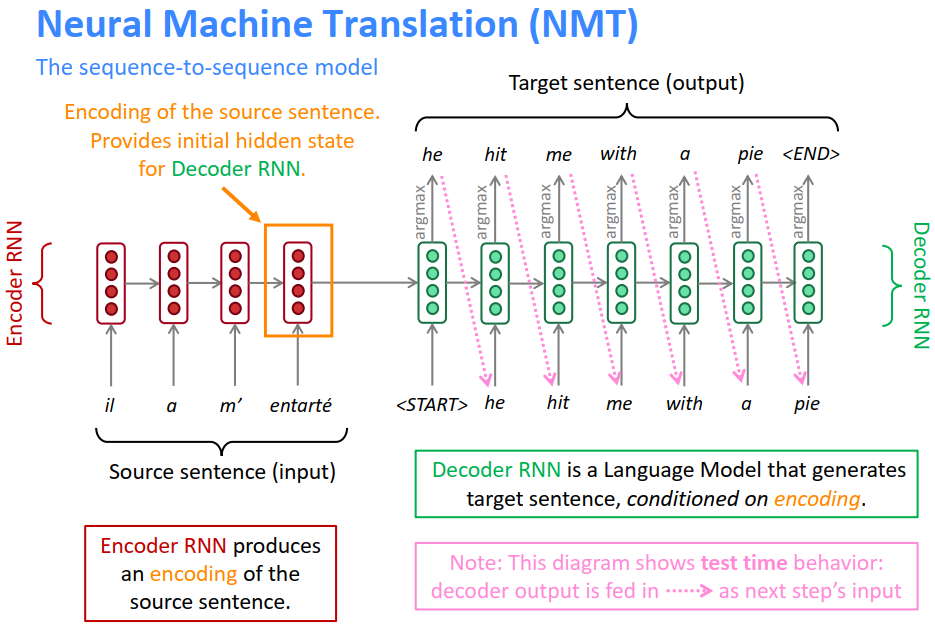
\includegraphics[width=0.8\linewidth]{fig/NMT.png}
\caption{seq2seq模型}
\label{fig:seq2seq}
\end{figure}

但在实际使用中,我们会使用Attention机制,如图\ref{fig:attention}所示。
这一部分会在下面编码器和解码器实现上详细说明。
\begin{figure}[H]
\centering
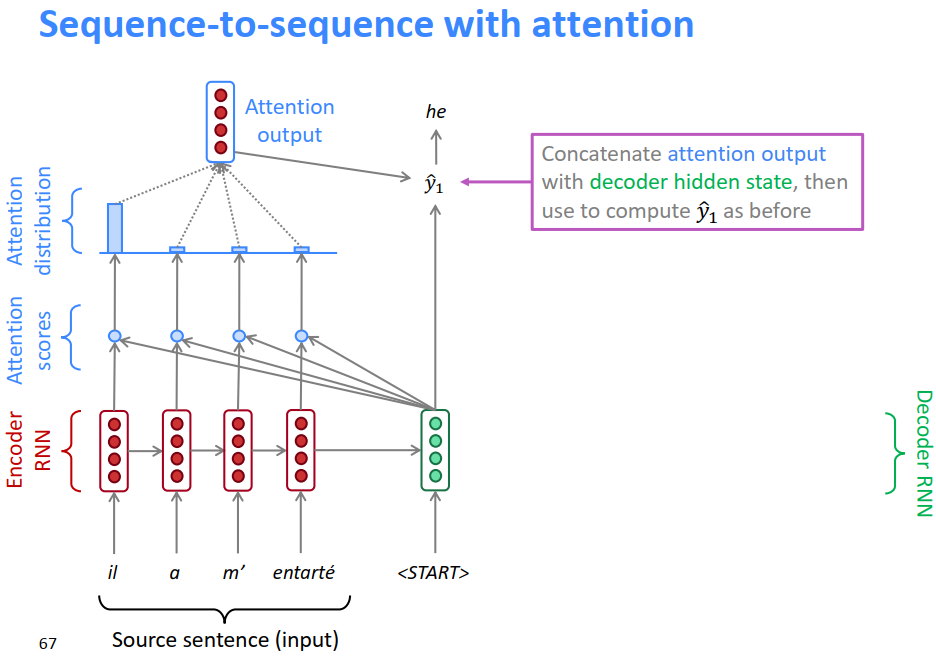
\includegraphics[width=0.8\linewidth]{fig/attention.png}
\caption{Attention机制}
\label{fig:attention}
\end{figure}

而这里的编码器和解码器采用LSTM进行搭建。
LSTM包括两个传递状态,如图\ref{fig:lstm-unit}所示\footnote{图源自Application of Long Short-Term Memory (LSTM) Neural Network for Flood Forecasting, \url{https://www.mdpi.com/2073-4441/11/7/1387}}。
这里要特别关注LSTM的输出$h_t$实际上就是当前的隐含状态,这一点在构造attention向量时特别有用。

\begin{figure}[H]
\centering
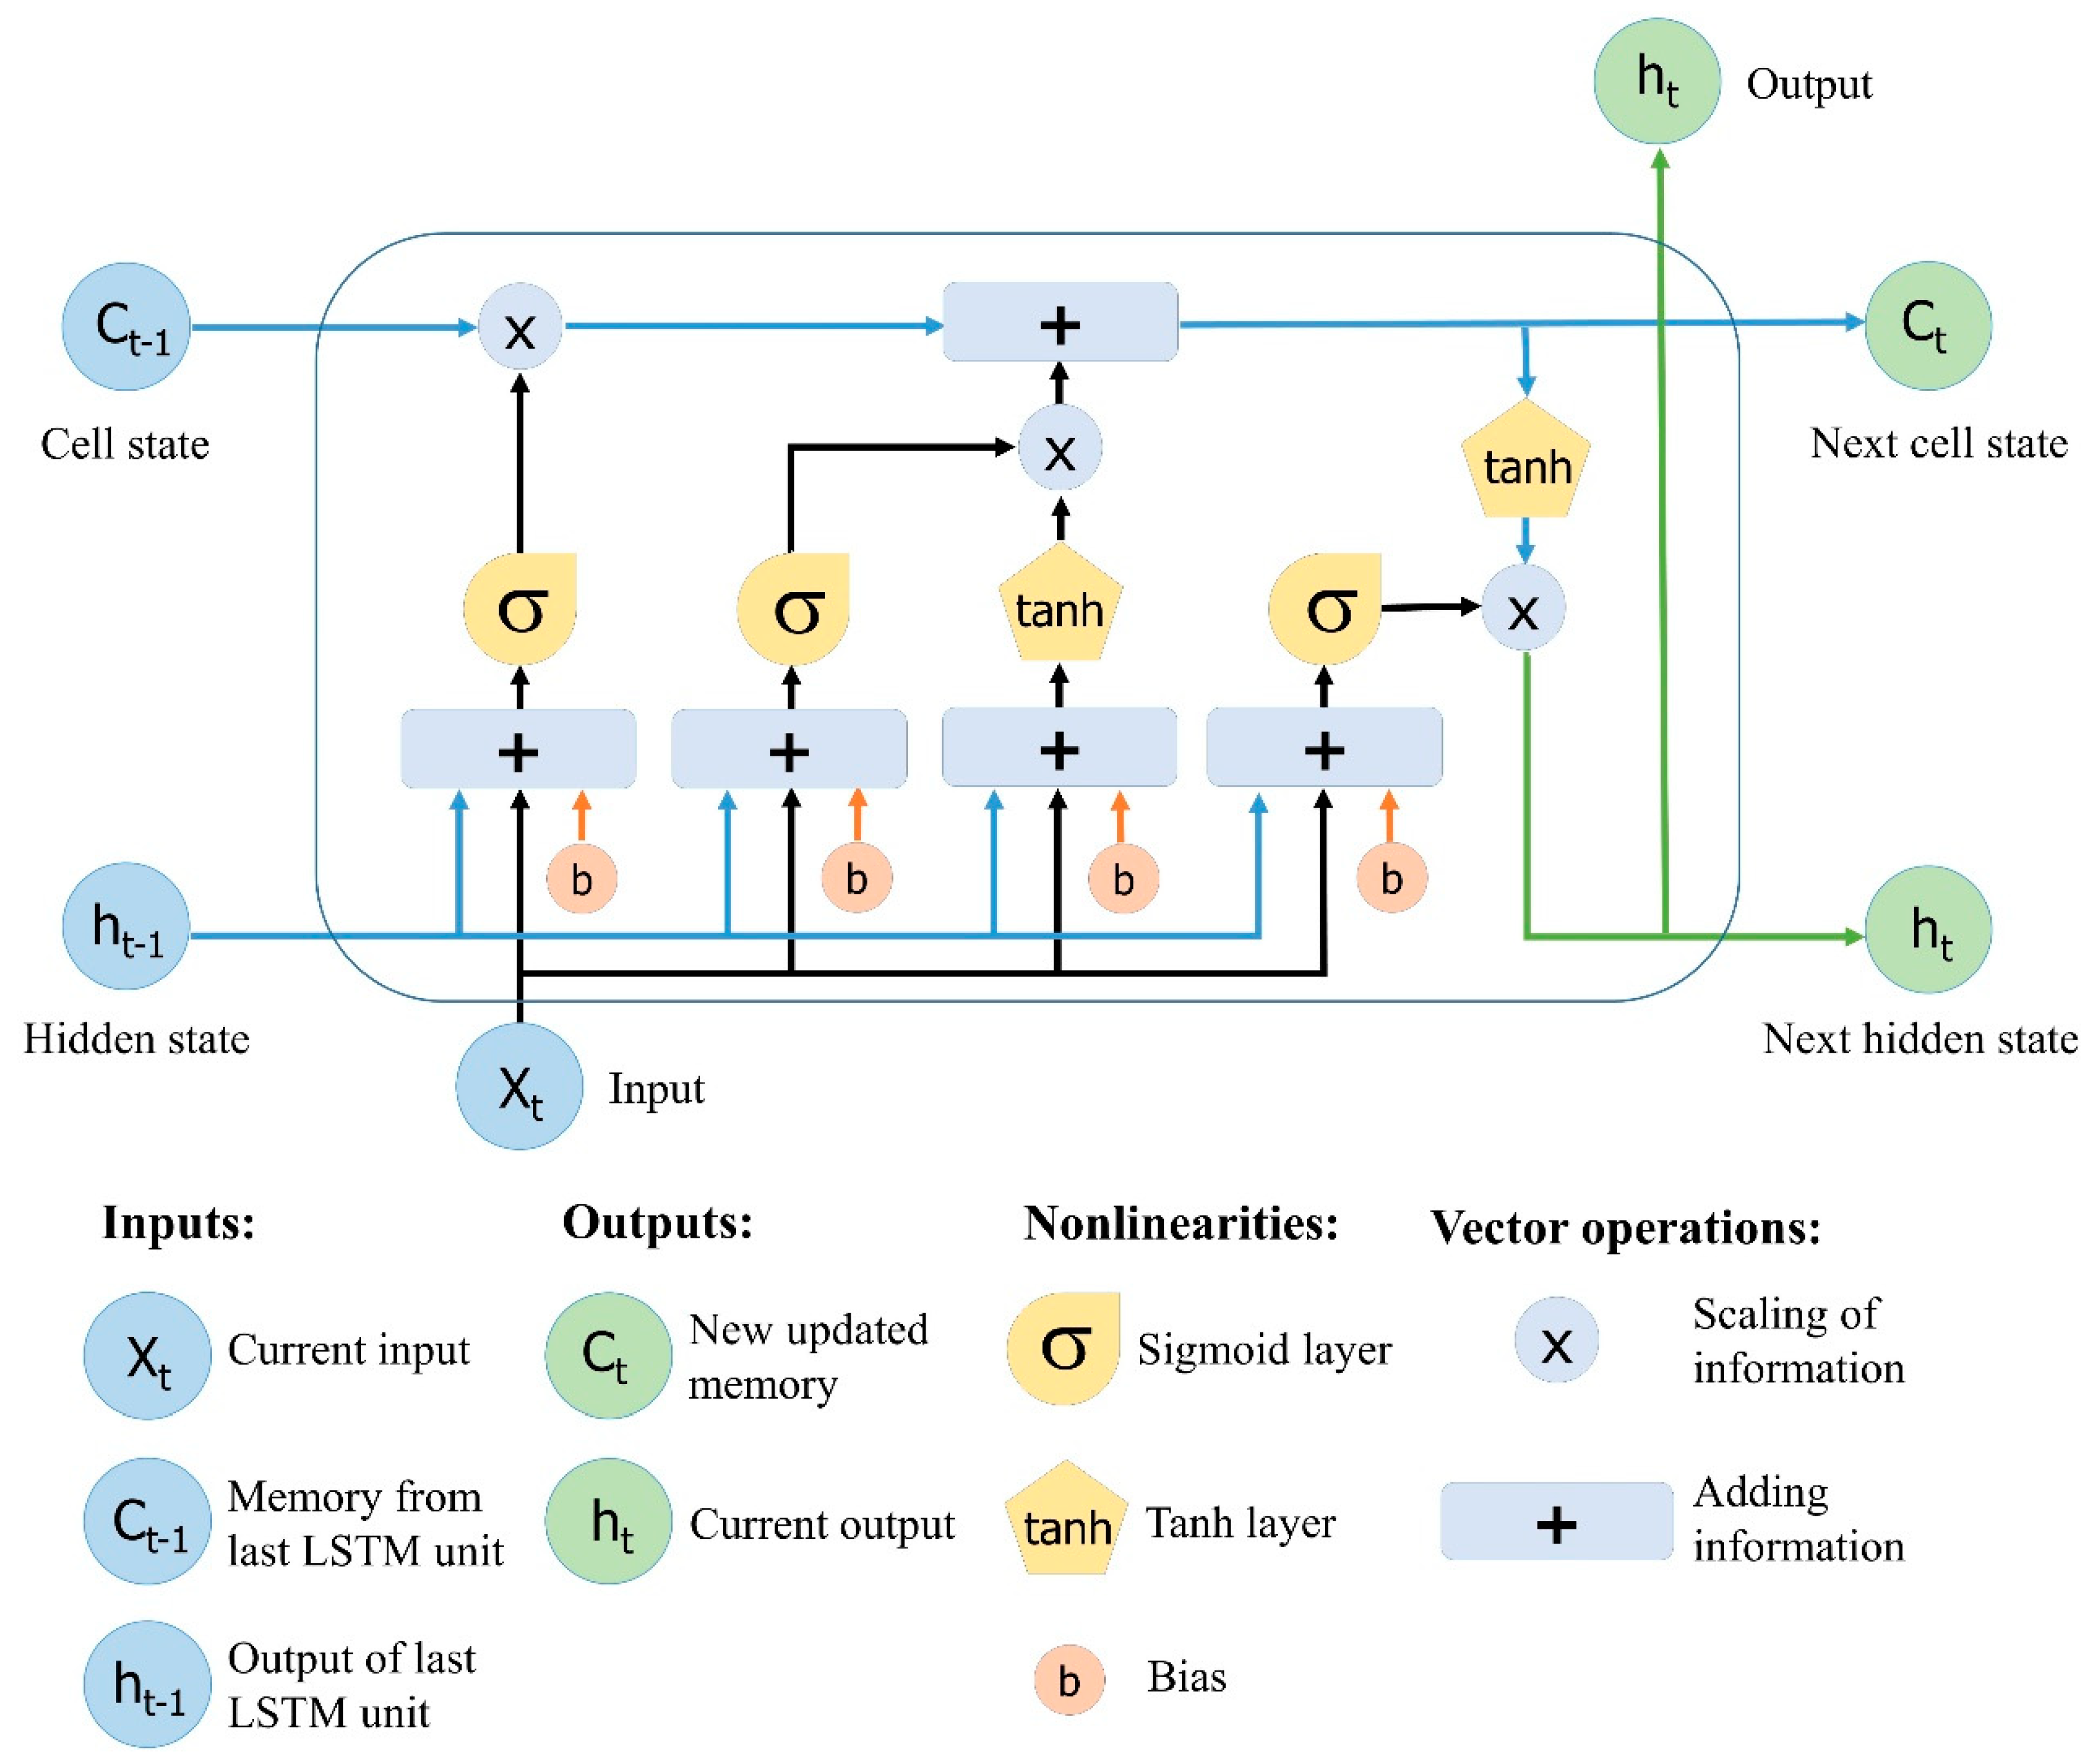
\includegraphics[width=0.8\linewidth]{fig/lstm-unit.png}
\caption{LSTM单元}
\label{fig:lstm-unit}
\end{figure}

下面将分别讲述编码器(encoder)和解码器(decoder)的详细搭建过程,采用的编程框架为Pytorch。

\subsection{编码器}
详细说明均已附在下面的代码注释中,并且给出了每一步操作的张量维度。
\begin{lstlisting}
class EncoderRNN(nn.Module):
    def __init__(self, input_size, hidden_size, dropout=0.1):
        super(EncoderRNN, self).__init__()
        self.input_size = input_size
        self.hidden_size = hidden_size
        self.dropout = dropout

        # embed = nn.Embedding(vocab_size, vector_size)
        # "vocab_size" is the number of words in your train, val and test set
        # "vector_size" is the dimension of the word vectors you are using
        # you can view it as a linear transformation
        # the tensor is initialized randomly
        # Input: (*), LongTensor of arbitrary shape containing the indices to extract (i.e. batch size)
        # Output: (*, H), where * is the input shape and H = embedding_dim
        self.embedding = nn.Embedding(input_size, hidden_size)
        # make the embedding size equal to the hidden dimension (lstm size)
        # batch_first makes it to (batch_size, seq_len, features)
        self.lstm = nn.LSTM(hidden_size, hidden_size, dropout=self.dropout, batch_first=True)

    def forward(self, x, prev_state, input_lengths):
        """
        x: (batch_size, seq_len)
            seq_len can be viewed as the time step (many small chunks)
        embedding: (batch_size, seq_len, embedding_size)
            since batch_first flag is set to True, the first dimension is batch_size
        output: (batch_size, seq_len, embedding_size)
        h_t: (1, batch_size, hidden_size) # Actually, 1 = num_layers*num_directions
        c_t: (1, batch_size, hidden_size)

        Pytorch's pack_padded_sequence can be used to
        tackle the problem of variable length sequences
        Packs a Tensor containing padded sequences of variable length.

        torch.nn.utils.rnn.pack_padded_sequence(input, lengths, batch_first=False, enforce_sorted=True)
        input can be of size T x B x * where T is the length of the longest sequence (equal to lengths[0]),
        B is the batch size, and * is any number of dimensions (including 0).
        If batch_first is True, B x T x * input is expected.

        Reference:
        * https://discuss.pytorch.org/t/understanding-lstm-input/31110/3
        * https://pytorch.org/docs/stable/nn.html#torch.nn.utils.rnn.PackedSequence
        * https://stackoverflow.com/questions/51030782/why-do-we-pack-the-sequences-in-pytorch
        * https://pytorch.org/docs/stable/notes/faq.html#pack-rnn-unpack-with-data-parallelism
        * https://gist.github.com/HarshTrivedi/f4e7293e941b17d19058f6fb90ab0fec
        """
        embedding = self.embedding(x)
        total_length = x.size(1) # max sequence length
        packed = torch.nn.utils.rnn.pack_padded_sequence(embedding, input_lengths, batch_first=True) # reduce computation
        output, state = self.lstm(packed, prev_state)
        output, output_lengths = torch.nn.utils.rnn.pad_packed_sequence(output, batch_first=True, total_length=total_length) # unpack (back to padded)
        return output, state

    def forward_without_padding(self, x, prev_state):
        embedding = self.embedding(x)
        output, state = self.lstm(embedding, prev_state)
        return output, state

    def initHidden(self,batch_size):
        return (torch.zeros(1, batch_size, self.hidden_size, device=device), # h_t
                torch.zeros(1, batch_size, self.hidden_size, device=device)) # c_t
\end{lstlisting}

编码器的传播(forward)过程比较简单,将输入向量(x)做词嵌入后,输入LSTM计算,即可得到输出和下一隐态。
输出之后将会被送到attention模块中,而隐态则会水平通过LSTM隐含层进行传递。

这里注意几个关键点:
\begin{itemize}
\item pytorch提供了词嵌入的语句,即\verb'nn.Embedding',可以实现从离散索引到高维空间词向量的映射
\item 由于RNN输入文本句子长度常常是不一致的,并不利于批训练,因此需要对句子进行填充(padding)处理(见\ref{sub:batch_generator}节),但是在具体训练中并不需要对这些填充部分也进行输入,因此pytorch提供了对应的RNN padding语句,可以实现只将非padding部分传入训练,以大幅提升训练速度,框架如下。
\begin{lstlisting}
packed = torch.nn.utils.rnn.pack_padded_sequence(embedding, input_lengths) # reduce computation
output, state = self.lstm(packed, prev_state)
output, output_lengths = torch.nn.utils.rnn.pad_packed_sequence(output) # unpack (back to padded)
\end{lstlisting}
\item 为了方便批处理,这里lstm的输入全部都要保证批(batch)的维度在第一维,即开启\verb'batch_first=True'模式
\end{itemize}

\subsection{解码器}
在解码器部分,我实现了两个版本,一个是传统的Seq2Seq中的解码器,即不添加attention部分。

\subsubsection{传统解码器}
\begin{lstlisting}
class DecoderRNN(nn.Module):
    def __init__(self, hidden_size, output_size):
        super(DecoderRNN, self).__init__()
        self.name = "Toy"
        self.hidden_size = hidden_size
        self.output_size = output_size

        self.embedding = nn.Embedding(output_size, hidden_size)
        self.lstm = nn.LSTM(hidden_size, hidden_size, batch_first=True)
        self.linear = nn.Linear(hidden_size, output_size)

    def forward(self, x, prev_state):
        """
        x: (batch_size, seq_len)
        embedding: (batch_size, seq_len, embedding_size) # embedding_size = hidden_size
            operate the words in embedding space
        output: (batch_size, seq_len, embedding_size)
        output: (batch_size, seq_len, output_size)
            from embedding space to index space
        h_t: (1, batch_size, hidden_size)
        c_t: (1, batch_size, hidden_size)
        """
        # outputs of the encoder are passed from hidden_state
        embedding = self.embedding(x)
        embedding = F.relu(embedding)
        output, state = self.lstm(embedding, prev_state)
        output = self.linear(output)
        return output, state

    def initHidden(self,batch_size):
        return (torch.zeros(1, batch_size, self.hidden_size, device=device), # h_t
                torch.zeros(1, batch_size, self.hidden_size, device=device)) # c_t
\end{lstlisting}

之所以要先搭建传统的解码器,一方面是构建起解码器的基本框架,另一方面则是测试整个seq2seq模型是否可以正常运作。
基本步骤和编码器类似,依然是读入词语,转为词嵌入表示,通过LSTM,最后经由线性层输出。

这里需要特别注意的是,由于后面训练时会采用交叉熵(CrossEntropyLoss),故这里的输出层不能采用softmax,因在Pytorch中已经将softmax函数封装在交叉熵函数中。

\subsubsection{Attention解码器}
添加了Attention模块的解码器则要复杂很多,这里的计算流程复现的是\cite{bib:luong}中的方法。

首先在时间步$t$通过上一步解码器的输出和上一步编码器的隐含层状态,计算当前时间步下解码器的隐含层状态$\vs_t\in\rr^h$。
又有时间步$t$下的编码器隐含层状态$\vh_1,\ldots,\vh_N\in\rr^h$,进而可以计算attention的权重分数
\[\ve=\bmat{\vs^\T\vh_1 & \cdots & \vs^\T\vh_N}\in\rr^N\]
通过取softmax得到这一步下的attention权重
\[\valpha^t=softmax(\ve^t)\in\rr^N\]
然后将权重与编码器隐含层状态相乘求和得到attention输出
\[\va_t=\sum_{i=1}^N\alpha^t_i\vh_i\in\rr^h\]
最终我们将attention的输出$\va_t$和解码器的隐含层状态$\vs_t$连接(concat)得到
\[[\va_t;\vs_t]\in\rr^{2h}\]
并通过一个线性层映射到输出词向量空间上,进而得到目标语言的词语向量表示。

完整模块如下,注意这里大量使用了矩阵运算。
为确保正确性,我将每一步的张量维度都标注在注释中。
其中\verb'torch.bmm'是Pytorch提供的\emph{批矩阵乘}函数,输入矩阵维度为$(b,m,n)$和$(b,n,p)$,则输出矩阵维度为$(b,m,p)$,这里的$b$即为批量大小。
\begin{lstlisting}
class AttnDecoderRNN(nn.Module):
    def __init__(self, hidden_size, output_size, dropout_p=0.1, max_length=32):
        super(AttnDecoderRNN, self).__init__()
        self.name = "Attn"
        self.hidden_size = hidden_size
        self.output_size = output_size
        self.dropout_p = dropout_p

        self.embedding = nn.Embedding(self.output_size, self.hidden_size)
        self.dropout = nn.Dropout(self.dropout_p)
        self.lstm = nn.LSTM(self.hidden_size, self.hidden_size, batch_first=True)
        self.linear = nn.Linear(self.hidden_size*2, self.output_size)

    def forward(self, x, prev_hidden, encoder_outputs):
        """
        x: (batch_size=32, seq_len=1, output_size)
        prev_hidden: (1, batch_size=32, hidden_size)
        encoder_outputs: (batch_size=32, seq_len=32, hidden_size) # encoder hidden states

        embedded: (batch_size=32, seq_len=1, hidden_size)
        decoder_output: (batch_size, seq_len=1, hidden_size)
        attn_score: dot(encoder_outputs,decoder_output)
            (batch_size,seq_len,1)
        attn_weights: softmax(attn_score)
            (batch_size,seq_len,1) -> (batch_size,1,seq_len)
        attn_output: dot(attn_weights,encoder_outputs)
            (batch_size,1,hidden_size)
        cat: cat(attn_output,decoder_output)
            (batch_size,1,2*hidden_size)
        output: (batch_size,1,output_size)
        """
        embedded = self.embedding(x)
        decoder_output, hidden = self.lstm(embedded, prev_hidden)
        attn_score = torch.bmm(encoder_outputs,decoder_output.transpose(1,2))
        attn_weights = F.softmax(attn_score,dim=1)
        attn_output = torch.bmm(attn_weights.transpose(1,2),encoder_outputs)
        cat = torch.cat((attn_output,decoder_output),dim=2)
        output = self.linear(cat)

        return output, hidden, attn_weights

    def initHidden(self,batch_size):
        return (torch.zeros(1, batch_size, self.hidden_size, device=device), # h_t
                torch.zeros(1, batch_size, self.hidden_size, device=device)) # c_t
\end{lstlisting}


\section{模型训练}
\subsection{批生成器}
\label{sub:batch_generator}
为了方便Pytorch模型的训练,我构造了一个\verb'TextDataset'的类,并继承了\verb'torch.utils.data.Dataset',其中封装了前文的初始化过程。

这里需要将长度超过字串长(seq\_len)的句子删除,然后总训练量按批大小取整,得到几个成员变量:
\begin{itemize}
    \item \verb'src_lang':源语言词表、索引映射等
    \item \verb'dst_lang':目标语言词表、索引映射等
    \item \verb'in_text':源语言输入句子(已将其索引离散化)
    \item \verb'out_text':目标语言输出句子(已将其索引离散化)
    \item \verb'pairs':平行语料
\end{itemize}

同时重载了\verb'__len__'和\verb'__getitem__'函数,用于构造生成一个批量的批量的训练数据。
\begin{lstlisting}
class TextDataset(data.Dataset):
    """
    My own text dataset
    ref: https://stanford.edu/~shervine/blog/pytorch-how-to-generate-data-parallel
    """
    def __init__(self,mode="train",dataset_size=10000,max_seq_len=32,batch_size=32,trunc=-1):
        self.src_lang, self.dst_lang, self.pairs = preprocess(mode,dataset_size)
        # too details, please see source code

    def __len__(self):
        """
        Return the total number of samples
        """
        return len(self.in_text)

    def __getitem__(self, idx):
        """
        Generate one sample of the data
        """
        x = self.in_text[idx]
        y = self.out_text[idx]
        x_len = self.src_len[idx]
        y_len = self.dst_len[idx]
        return x, y, x_len, y_len
\end{lstlisting}

注意这里\verb'__getitem__'函数还返回了输入和输出句子的长度,用于\verb'pack_padded_sequence'的输入。

具体调用则通过下面两条语句调用,后一条语句即批训练迭代器,每次进行枚举时会返回一个批样本。
\begin{lstlisting}
train_set = TextDataset("train",10000)
train_loader = data.DataLoader(dataset=train_set,batch_size=flags.batch_size,shuffle=True)
\end{lstlisting}

\subsection{单轮迭代}
在每轮训练中,按照以下步骤进行操作:
\begin{enumerate}
    \item 从\verb'train_loader'中取出一个批次,得到输入向量$x$和目标向量$y$
    \item 将优化器梯度归零\verb'zero_grad'
    \item 对输入向量$x$按照批次内每条句子的长度降序排序,方便输入\verb'pack_padded_sequence'
    \item 将$x$输入编码器得到编码器输出\verb'encoder_outputs'和编码器隐状态(由于是批训练,而且Pytorch已经封装了时间步上的多步操作,故只需调用\verb'lstm.forward'一行语句即可)
    \item 将编码器隐态传递给解码器,解码器第一个输入为\verb'<BOS>',如果设置了attention,则还需将编码器的所有隐态输出传递给解码器
    \item 解码器需要\textbf{一步一步}进行迭代
    \begin{itemize}
        \item 若采用了Teacher forcing,则每个时间步上的输入为正确目标句子中的词语
        \item 如果不采用Teacher forcing,则将当前步的输出作为下一步的输入
    \end{itemize}
    这里通过\verb'teacher_forcing_ratio'进行调节
    \item 当到最大序列长或输出为\verb'<EOS>'时停止当前批次的输出
    \item Loss计算并回传
    \item 为避免梯度回传时经过LSTM的隐态$h_t$和$c_t$,故需要将其\verb'detach',这一步是Pytorch搭建RNN中非常关键的一步,否则会引起梯度图爆炸、重复梯度计算的问题
\end{enumerate}

核心代码部分如下:
\begin{lstlisting}
    for e in range(num_epochs):
        encoder_ht, encoder_ct = encoder.initHidden(batch_size)
        decoder_ht, decoder_ct = decoder.initHidden(batch_size)

        for step, (x, y, x_len, y_len) in enumerate(train_loader):
            iteration += 1
            encoder.train()
            decoder.train()

            encoder_optimizer.zero_grad()
            decoder_optimizer.zero_grad()
            seq_lengths, perm_idx = torch.tensor(x_len).sort(0,descending=True)

            x = torch.tensor(x).to(torch.int64).to(device) # (batch_size, seq_size)
            y = torch.tensor(y).to(torch.int64).to(device) # (batch_size, seq_size)
            x = x[perm_idx]
            y = y[perm_idx]

            encoder_outputs, (encoder_ht, encoder_ct) = encoder(x, (encoder_ht, encoder_ct), seq_lengths)

            decoder_input = torch.tensor([BOS_token] * batch_size).reshape(batch_size,1).to(device) # <BOS> token
            decoder_ht, decoder_ct = encoder_ht, encoder_ct # use last hidden state from encoder

            # run through decoder one time step at a time
            max_dst_len = y.shape[1]
            all_decoder_outputs = torch.zeros((max_dst_len,flags.batch_size,decoder.output_size))
            if random.random() < flags.teacher_forcing_ratio:
                for t in range(max_dst_len): # for each time step
                    if decoder.name == "Toy":
                        # decoder_output: (batch_size, seq_len, output_size)
                        decoder_output, (decoder_ht, decoder_ct) = decoder(decoder_input, (decoder_ht, decoder_ct))
                        all_decoder_outputs[t] = decoder_output.transpose(1,0)
                    elif decoder.name == "Attn":
                        decoder_output, (decoder_ht, decoder_ct), decoder_attn = decoder(decoder_input, (decoder_ht, decoder_ct), encoder_outputs)
                        all_decoder_outputs[t] = decoder_output.transpose(1,0)
                    else:
                        decoder_output, (decoder_ht, decoder_ct), decoder_attn = decoder(decoder_input, (decoder_ht, decoder_ct), encoder_outputs)
                        all_decoder_outputs[t] = decoder_output
                    # teaching forcing: next input is the current target
                    decoder_input = y[:,t].reshape(batch_size,1) # remember to reshape
            else: # without teacher forcing
                for t in range(max_dst_len): # for each time step
                    if decoder.name == "Toy":
                        # decoder_output: (batch_size, seq_len, output_size)
                        decoder_output, (decoder_ht, decoder_ct) = decoder(decoder_input, (decoder_ht, decoder_ct))
                        all_decoder_outputs[t] = decoder_output.transpose(1,0)
                    elif decoder.name == "Attn":
                        decoder_output, (decoder_ht, decoder_ct), decoder_attn = decoder(decoder_input, (decoder_ht, decoder_ct), encoder_outputs)
                        all_decoder_outputs[t] = decoder_output.transpose(1,0)
                    else:
                        decoder_output, (decoder_ht, decoder_ct), decoder_attn = decoder(decoder_input, (decoder_ht, decoder_ct), encoder_outputs)
                        all_decoder_outputs[t] = decoder_output
                    # use the current output as the next input
                    topv, topi = decoder_output.topk(1)
                    decoder_input = topi.squeeze().detach().reshape(batch_size,1)
#                     if decoder_input.item() == EOS_token: # cannot add for batch training!
#                         break

            # loss calculation
            # (max_dst_len, batch_size, output_size)
            # (batch_size, max_dst_len, output_size)
            # (batch_size, output_size, max_dst_len)
            loss = criterion(all_decoder_outputs.permute(1,2,0).to(device).to(device), y) # transpose(1,0).transpose(1,2)

            loss_value = loss.item()

            loss.backward()

            # avoid delivering loss from h_t and c_t
            # thus need to remove them from the computation graph
            encoder_ht, encoder_ct = encoder_ht.detach(), encoder_ct.detach()
            decoder_ht, decoder_ct = decoder_ht.detach(), decoder_ct.detach()

            # avoid gradient explosion
            _ = torch.nn.utils.clip_grad_norm_(encoder.parameters(), flags.gradients_norm)
            _ = torch.nn.utils.clip_grad_norm_(decoder.parameters(), flags.gradients_norm)

            # update parameters with optimizers
            encoder_optimizer.step()
            decoder_optimizer.step()

            losses.append(loss_value)

            # print and save model, see source code

        # learning rate decay
        encoder_scheduler.step()
        decoder_scheduler.step()
\end{lstlisting}

注意这里忽略了大部分输出和保存模块,欲知详情请见源代码。
其中一些优化器和附加方法说明如下:
\begin{itemize}
    \item 损失函数:CrossEntropyLoss
    \item 优化器:编码器和解码器都采用Adam
    \item 学习率衰减:采用分段线性函数,迭代一定轮数后对学习率进行衰减,以避免学习停滞
    \item 梯度裁剪:为避免梯度爆炸,采用了gradient clipping机制
\end{itemize}

\subsection{其他实现细节}
\begin{itemize}
    \item 采用\verb'argparse'进行命令行参数的读入与操作(主要是一些模型的超参数及文件路径)
    \item 采用\verb'logging'模块对训练过程进行日志记录,以便跟踪存在的问题
    \item 采用\verb'time'模块对模型训练时间进行记录,同时可以预测剩余训练时间
    \item 采用\verb'torch.save(net.state_dict())'的方法保存模型参数,一方面可以防止训练过程中的模型丢失,另一方面又可以避免将整个模型存储下来的空间开销
\end{itemize}

\section{模型预测}
模型预测我同样采用了两种方法,一种直接选取最大预测值输出,另一种则采用集束搜索(Beam Search)方法。

与训练时一样,源语言句子还是直接一整句丢入编码器中,然后\textbf{逐时间步}迭代解码器。
在评价时没有采用批处理,即每个批大小为1。

\subsection{最大预测值输出}
在每一时间步都选取解码器的最大预测值进行输出,只需调用Pytorch的topk函数即可。
得到离散索引后,再将其映射回目标词语,一步步迭代即得到翻译出来的目标句子。

\subsection{集束搜索(Beam Search)}
集束搜索的示意图如\ref{fig:beam_search}所示,每次保留集束宽度(beam width)$w$个扩展,以探索更多的可能性。其主要基于最大似然估计方法,路径的评价函数如下
\[score(y_1,\ldots,y_t)=\log P_{LM}(y_1,\ldots,y_t\mid x)=\sum_{i=1}^t\log P_{LM}(y_i\mid y_1,\ldots,y_{i-1},x)\]
\begin{figure}[H]
\centering
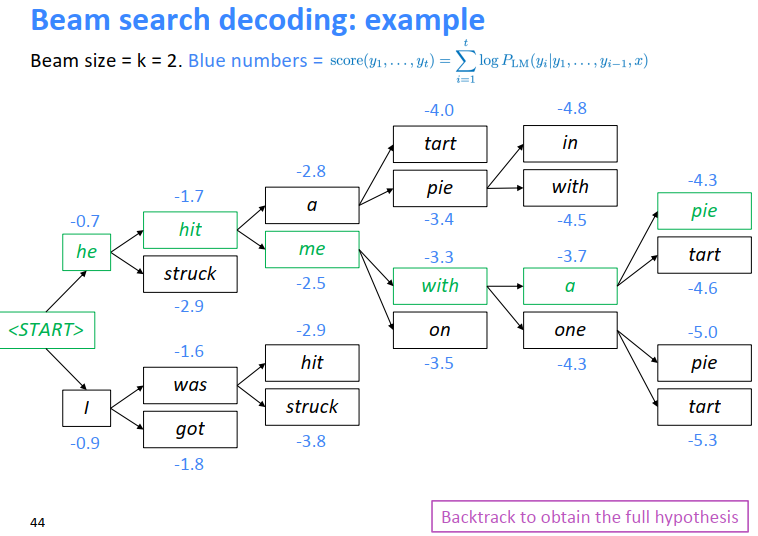
\includegraphics[width=0.8\linewidth]{fig/beam_search.png}
\caption{集束搜索(Beam Search)}
\label{fig:beam_search}
\end{figure}

仔细分析一下实现起来也不是很麻烦,关键是要注意到,扩展出来的结点数目最大为$w^2$个,那么每次只用记录这$w^2$个扩展,并且从中选取最优的$w$个出来作为下一轮迭代的父节点即可。
由于Pytorch提供了\verb'topk'函数,因此可以很方便地选取出最高的$w$个累积概率值。

同时注意由于不同路径的词语数目不一致,可能导致长的句子比较有优势,因此采用归一化方法
\[score(y_1,\ldots,y_t)=\frac{1}{t^\alpha}\sum_{i=1}^t\log P_{LM}(y_i\mid y_1,\ldots,y_{i-1},x)\]
其中$\alpha$为归一化因子,一般设为$1$即可。

\subsection{单轮预测代码}
\begin{lstlisting}
from nltk.translate.bleu_score import SmoothingFunction, sentence_bleu
# https://cloud.tencent.com/developer/article/1042161

def evalOne(in_text, out_text, src_lang, dst_lang, encoder, decoder, beam_search=False, beam_width=2, print_flag=False):
    if len(in_text) > flags.seq_size or len(out_text) > flags.seq_size:
        return None, None, -1
    encoder.eval() # set in evaluation mode
    decoder.eval()

    in_text, in_text_len = in_text
    x = torch.tensor(in_text).to(device).reshape(1,-1)
    seq_len = torch.tensor([in_text_len]).to(torch.int64).to(device)
    # encoder
    encoder_ht, encoder_ct = encoder.initHidden(1)
    encoder_outputs, (encoder_ht, encoder_ct) = encoder(x, (encoder_ht, encoder_ct), seq_len)

    decoder_input = torch.tensor([BOS_token] * 1).reshape(1,1).to(device) # <BOS> token
    decoder_ht, decoder_ct = encoder_ht, encoder_ct # use last hidden state from encoder

    # decoder
    # run through decoder one time step at a time
    max_len = int(flags.seq_size*1.5)
    decoder_attentions = torch.zeros(max_len,flags.seq_size)
    if not beam_search:
        decoded_words = []
        decoded_index = []
        for t in range(max_len):
            if decoder.name == "Toy":
                decoder_output, (decoder_ht, decoder_ct) = decoder(decoder_input, (decoder_ht, decoder_ct))
            elif decoder.name == "Attn":
                decoder_output, (decoder_ht, decoder_ct), decoder_attn = decoder(decoder_input, (decoder_ht, decoder_ct), encoder_outputs)
                decoder_attentions[t] = decoder_attn.transpose(1,2).squeeze(0).squeeze(0).cpu().data
#                 print(sum(decoder_attentions[t]))
            else:
                decoder_output, (decoder_ht, decoder_ct), decoder_attention = decoder(decoder_input, (decoder_ht, decoder_ct), encoder_outputs)
                decoder_attentions[t,:decoder_attention.size(2)] += decoder_attention.squeeze(0).squeeze(0).cpu().data
            # choose top word from output
            top_value, top_index = decoder_output.data.topk(1)
            ni = top_index[0][0].item()
            decoded_index.append(ni)
            word = dst_lang.index2word[ni]
            decoded_words.append(word)
            if word == "<EOS>":
                break
            decoder_input = torch.LongTensor([ni]).reshape(1,1).to(device)
    else:
        """
        Beam seach:
        https://medium.com/@dhartidhami/beam-search-in-seq2seq-model-7606d55b21a5
        """
        path = [(BOS_token,0,[])] # input, value, words on the path
        for t in range(max_len):
            new_path = []
            flag_done = True
            for decoder_input, value, indices in path:
                if decoder_input == EOS_token:
                    new_path.append((decoder_input,value,indices))
                    continue
                elif len(path) != 1 and decoder_input in [BOS_token,PAD_token]:
                    continue
                flag_done = False
                decoder_input = torch.tensor([decoder_input]).reshape(1,1).to(device)
                if decoder.name == "Toy":
                    decoder_output, (decoder_ht, decoder_ct) = decoder(decoder_input, (decoder_ht, decoder_ct))
                elif decoder.name == "Attn":
                    decoder_output, (decoder_ht, decoder_ct), decoder_attn = decoder(decoder_input, (decoder_ht, decoder_ct), encoder_outputs)
                    decoder_attentions[t] = decoder_attn.transpose(1,2).cpu().data
                else:
                    decoder_output, (decoder_ht, decoder_ct), decoder_attention = decoder(decoder_input, (decoder_ht, decoder_ct), encoder_outputs)
    #                 decoder_attentions[t,:decoder_attention.size(2)] += decoder_attention.squeeze(0).squeeze(0).cpu().data
                # choose top word from output
                softmax_output = F.log_softmax(decoder_output,dim=2) # dim 2!
                top_value, top_index = softmax_output.data.topk(beam_width)
                top_value = top_value.cpu().squeeze().numpy() + value
                top_index = top_index.cpu().squeeze().numpy()
                for i in range(beam_width):
                    ni = int(top_index[i])
                    new_path.append((ni,top_value[i],indices+[ni]))
            if flag_done:
                _, value, decoded_index = new_path[0]
                break
            else:
                new_path.sort(key=lambda x:x[1]/len(x[2])**0.7,reverse=True) # normalization
                path = new_path[:beam_width]

        if not flag_done:
            _, value, decoded_index = path[0]
        decoded_words = []
        for ni in decoded_index:
            word = dst_lang.index2word[ni]
            decoded_words.append(word)

    pad_index = np.where(out_text == PAD_token)
    if len(pad_index[0]) == 0:
        pad_index = len(out_text)
    else:
        pad_index = pad_index[0][0]
    filter_outtext = list(filter("<PAD>".__ne__,out_text[:pad_index]))
    decoded_index = list(filter("<PAD>".__ne__,decoded_index))
    sm = SmoothingFunction()
    bleu = sentence_bleu([filter_outtext],decoded_index,smoothing_function=sm.method4)
    if print_flag:
        print(out_text[:pad_index])
        print(decoded_index)
        print("Bleu score: {}".format(bleu))
        res_words = " ".join(decoded_words)
        print("< {}".format(src_lang.getSentenceFromIndex(in_text)))
        print("= {}".format(dst_lang.getSentenceFromIndex(filter_outtext)))
        print("> {}".format(res_words))
        print()
    return decoded_words, decoder_attentions[:t+1, :flags.seq_size], bleu
\end{lstlisting}

\section{实验结果}
训练的Loss函数

集束搜索的时间成本太高

最终得到BLUE-4的指标为

\section{实验心得}
本学期的课程终于结束了,通过两次实验充分体会到了NLP的基本原理与方法。

训练时间、训练成本太大了

虽然说现在深度学习的兴起,给NLP巨大的发展空间,但是其能达到的水平还是极大依赖于人工的。
还是那句话,``有多少人工就有多少智能''。

硬编码规则

人工预处理

\begin{thebibliography}{99}
\bibitem{bib:unicode} Unicode字符百科,\url{https://unicode-table.com/cn/blocks/cjk-unified-ideographs/}
\bibitem{bib:stem} Stemming and Lemmatization, \url{https://nlp.stanford.edu/IR-book/html/htmledition/stemming-and-lemmatization-1.html}
\bibitem{bib:luong} Minh-Thang Luong, Hieu Pham, and Christopher D. Manning, \emph{Effective Approaches to Attention-based Neural Machine Translation}, EMNLP, 2015
\end{thebibliography}

\end{document}
% 平台:Pytorch, Tensorflow or Keras…
% 模型要求:
% 两个LSTM分别作为Encoder和Decoder
% 实现基于注意力机制的机器翻译
% 自行选择分词工具
% 改变teacher forcing ratio,观察效果
% Beam Search策略
% 评估指标:BLEU值(BLEU-4)
% 词向量:随机初始化或自选预训练词向量
% 设备:CPU/GPU

% 要求:
% 1. 描述清楚核心代码逻辑和tensor维度
% 2. 描述清楚代码的运行环境和软件版本
% 3. 独立完成,不得抄袭!不得抄袭!不得抄袭

% 参考教程:
% pytorch.org/tutorias/intermediate/seq2seq_translation_tutorial.html
% tensorflow.google.cn/tutorials/text/nmt_with_attention

% 相关论文:
% Effective Approaches to Attention-based Neural Machine Translation, Luong et al., EMNLP 2015
% Neural Machine Translation by Jointly Learning to Align and Translate, Bahdanau et al., ICLR 2015
% Bleu: a Method for Automatic Evaluation for Machine Translation, Papineni et al., ACL 2002